
% !TeX spellcheck = en_US
\documentclass[12pt, onecolumn]{article}

\usepackage{graphicx}

%opening
\title{Advanced Machine Learning - Assignment 5}
\author{Pranav Kasela \\$846965$}
\date{}
\begin{document}

\maketitle
\section*{Introduction}
The objective of this assignment is to use the SMBO models to find the hyperparameters of a Multi Layer Perceptron which maximizes the accuracy on a 10 folds cv.
The language used in this assignment is python with the SMAC package for the Hyperparameter optimization and Sklearn for the MLPerceptron.
Actually there is another easier package based on SMAC called `auto-sklearn', but in this assignment the basic SMAC package was used.
The dataset has 9 features and 1 target, the 9 features are apparently numeric, but the documentation explains that the variable V1 is the Season, which assumes the following values: $-1$:`winter', $-0.33$:`spring', $0.33$:`summer', $1.0$:`fall', since they are cyclic variable it cannot be considered completely correct to use ordered variable from $-1$ to $+1$, thus a one hot encoding is performed, another variable which cannot be considered equidistantly ordered is the V7 (Frequency of alcohol consumption), V7 assumes the following 5 values: $0.2$:`several times a day', $0.4$:`every day',$0.6$:`several times a week',  $0.8$:`once a week',$1.0$:`hardly ever never', a one hot encoding is also performed in this case.\\
This is the only basic preprocessing done on the data, the other values were accepted as numeric since they had mostly 2 or 3 classes or were already normalized.

\section*{SMAC}
The next step was to create a ``Wrapper'' around the SMAC package, just for our task (so it won't generalize well to other problems), this made the code easier for all the exercise.
The wrapper is named ``optimizer'' and it takes in input the surrogate model name (`rf', `gp') and will create SMAC4BO for the `gp' model and SMAC4HPO for the `rf' model, configuration space object containing information regarding, objective function which needs to be minimized, acquisition function name which can be `EI', `LCB' or `PI', number of iterations, initial points and an eventual seed.\\
The optimizer function creates every object necessary for SMAC: Scenario, AcquisionFunction, SMAC Objects etc., the code is commented in a very detailed way\footnote{Well surely better than the SMAC documentation.} so how the function works will not be explained here, the optimizer function return an optimized SMAC object with it's history.
The function uses RandomConfigurations to create the initial design, and its seed is the same as the SMAC object, so all the SMAC models with the same number of initial point will have the same performance on the initial points, and since a seed (123456789) is fixed for most of the randomness for reproducibility, so the model can be considered deterministic.
The objective function in SMAC can only be minimized so instead of weighted accuracy, $1 -$ weighted accuracy is used.
\section*{First Exercise}
For the First configuration a Configuration Space is created and it consists of two parameters the `learning\_rate\_init' with range between $0.01$ and $0.1$ and `momentum'  with range between $0.1$ and $0.9$, the metric used is an weighted accuracy, the weights of each class are the relative frequency of the other class, so the class `Normal' has a weight of $0.12$ and the class `Altered' (the rare one) has a weight of $0.88$, this choice tackles the class imbalance problem with such a low number of data which, since such small number of data makes the oversampling technique somehow problematic.\\
The `GP' surrogate model (SMAC4BO) is chosen for this part, and the acquisition functions `EI', `LCB' and `PI' are used with $5$ initial points, and the iterations are set to $25 (20 + 5$ initial$)$.
While for the GridSearch evenly distributed points are taken from the Configuration Domains (5 for each parameter), and RadomSearch searches random points by itself.
The MultiLayer perceptron classifier has two hidden layers with 4 and 2 neurons respectively and all the other configuration are the default one, except for the seed which is fixed to have consistent results. 
In the table \ref{tab:Ex1_res} are the result of the different acquisition function and models\footnote{The time values might differ a little in the submitted notebook because of the small randomnesses in the time measurement}.
Even though SMAC minimized the error, the weighted accuracy is used for the scores and plots to make them more intuitive.

\begin{table}[!h]
  \centering
  \begin{tabular}{ |c|c|c|c|c|c| } 
    \hline
    Acquisitions/Models$\to$ & LCB  & EI & PI & Random & Grid \\
    \hline
    Time(seconds) & 90.84 & 98.68 & 92.35 & 6.94 & 6.72\\
    \hline
    Score(weighted accuracy) & 0.582 & 0.580 & 0.580 & 0.580 & 0.544\\ 
    \hline
  \end{tabular}
  \caption{Results of the First Exercise}
  \label{tab:Ex1_res}
\end{table}

\begin{figure}[!h]
  \centering
  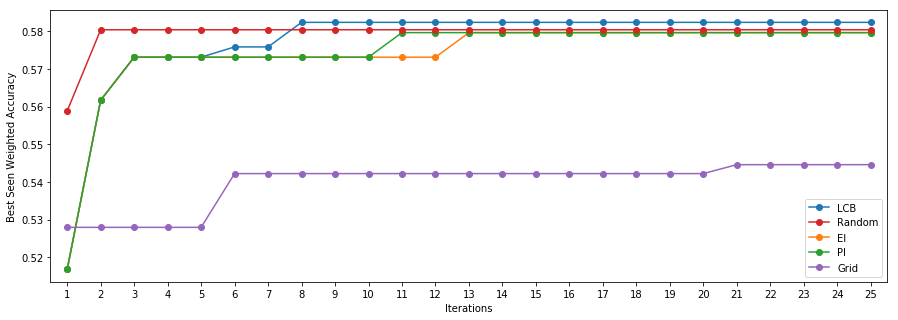
\includegraphics[width=\linewidth, height=5cm]{imgs/first.png}
  \caption{Plot of the result of the First Exercise}
  \label{fig:first}
\end{figure}
From the Table \ref{tab:Ex1_res} and Figure \ref{fig:first}, the best performance is obtained by the GP model with LCB as an acquisition function followed by the RandomSearch, which was fortunate enough to find the it's best configuration at the second iteration, the GP model with EI and PI have the same result and their score is very similar to the RandomSearch (it only differs of $0.0008$), while the worst performance is obtained by the GridSearch. In the Figure \ref{fig:first} all the GP model have the same starting point while Grid and Randomized Search starts at different initial points.
The best configuration found is with a learning rate of $0.06690282$ and a momentum $0.20195706$ and in the Table \ref{tab:best_1} its performance on a 10-CV is reported.
\begin{table}[!h]
  \centering
  \begin{tabular}{ |c|c|c|c|c|c| } 
    \hline
    Metrics& F1 & Precision & Recall & F1 Macro & Accuracy\\
    \hline
    Score& 0.173 & 0.133 & 0.250 & 0.536 & 0.823\\
    \hline
  \end{tabular}
  \caption{Results of 10-CV of the Best Configuration for the First Exercise}
  \label{tab:best_1}
\end{table}

\section*{Second Exercise}
The surrogate model is changed to the RandomForest (SMAC4HPO) Two more hyperparameters are added to the configuration space, the number of neurons of the first and second hidden layer, both with a range between $1$ and $5$, $10$ random initial points are chosen and the number of iteration is increased to $110 (100 + 10$ initial$)$.
The Random and Grid models are used too, here the two configurations for the hidden layer size is merged into a single configuration called hidden layer size and it is a tuple of 2 numbers ranging from 1 to 5.
While for the Random configuration obtaining $110$ iterations is easy, for the Grid Search 5 parameters from each configuration is chosen (5 for the learning rate, 5 for the momentum and 5 for the hidden layer sizes) obtaining 125 iterations, for the plot only the last 110 iterations are considered (just to make sure each algorithm has the same length).   
\begin{table}[!h]
  \centering
  \begin{tabular}{ |c|c|c|c|c|c| } 
    \hline
    Acquisitions/Models$\to$ & LCB  & EI & PI & Random & Grid \\
    \hline
    Time(seconds) & 242.27 & 211.60 & 210.63 & 23.35 & 22.04\\
    \hline
    Score(weighted accuracy) & 0.601 & 0.645 & 0.601 & 0.614 & 0.594\\ 
    \hline
  \end{tabular}
  \caption{Results of the Second Exercise}
  \label{tab:Ex2_res}
\end{table}

\begin{figure}[!h]
  \centering
  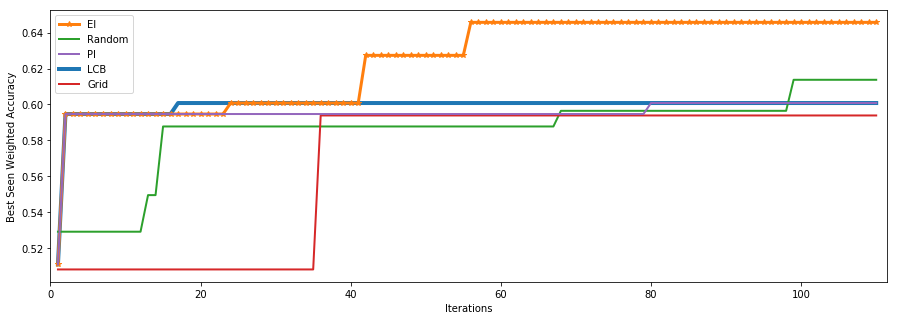
\includegraphics[width=\linewidth, height=5cm]{imgs/second.png}
  \caption{Plot of the result of the Second Exercise}
  \label{fig:second}
\end{figure}

\begin{table}[!h]
  \centering
  \begin{tabular}{ |c|c|c|c|c|c| } 
    \hline
    Metrics& F1 & Precision & Recall & F1 Macro & Accuracy\\
    \hline
    Score& 0.300 & 0.300 & 0.300 & 0.626 & 0.911\\
    \hline
  \end{tabular}
  \caption{Results of 10-CV of the Best Configuration for the Second Exercise}
  \label{tab:best_2}
\end{table}

\section*{Conclusions}
% time of algorithm
% best algorithm
% why chose the new metric
% what happens if we use always accuracy <- plot of second_accuracy
% reason why the time of Grid and Random is so low (parallel computation)
% does new metric improve the pure accuracy
% update the time is the tables

\end{document}